\section[Git]{Version control using git}
\begin{frame}
	\framesubtitle{Sharing the code}
	\begin{columns}
		\begin{column}{0.5\textwidth}
			\begin{itemize}[<+->]
				\item The code can easily be shared online on GitHub	
				\item Everyone can access and download the code
				\item Readme and wiki for documenting the code
				\item Issue tracker for reporting bugs and discussing the code
			\end{itemize}
		\end{column}
		\begin{column}{0.5\textwidth}
			\begin{figure}
				\includegraphics<1>[width=\textwidth]{./pictures/GitHub_frontpage.png}
				\includegraphics<2>[width=\textwidth]{./pictures/GitHub_online_and_download.png}
				\includegraphics<3>[width=\textwidth]{./pictures/GitHub_document.png}
				\includegraphics<4>[width=\textwidth]{./pictures/GitHub_issues.png}
			\end{figure}
		\end{column}
	\end{columns}
\end{frame}
\begin{frame}
	\frametitle{Getting rid of the old files using git}
	\begin{columns}
		\begin{column}{0.5\textwidth}
			\begin{itemize}[<+->]
				\item Download the GitHub repository using a GUI or the terminal.
				\item Find the files and delete them.
				\item The GUI informs you that changes have been made.
				\item The changes have to be staged.
				\item Write a commit message and commit the change.
				\item Our local version is now ahead of the GitHub version and the changes can be pushed.
				\item The versions are now identical
			\end{itemize}
		\end{column}
		\begin{column}{0.5\textwidth}
			\begin{figure}
				\includegraphics<1>[width=\textwidth]{./pictures/git_ext.png}
				\includegraphics<2>[width=\textwidth]{./pictures/delete.png}
				\includegraphics<3>[width=\textwidth]{./pictures/changes.png}
				\includegraphics<4>[width=\textwidth]{./pictures/stage_files.png}
				\includegraphics<5>[width=\textwidth]{./pictures/commit.png}
				\includegraphics<6>[width=\textwidth]{./pictures/commited.png}
				\includegraphics<7>[width=\textwidth]{./pictures/pushed.png}
			\end{figure}
		\end{column}
	\end{columns}
\end{frame}
\section[Code guidelines]{Making the code more readable}
\begin{frame}
	\frametitle{General tips on making code better}
	\begin{columns}
		\begin{column}{0.5\textwidth}
			\begin{itemize}
				\item Use descriptive variable names
				\item Have some space in between lines
				\item Write comments
				\item Write docstrings
				\item Don't copy and paste code
			\end{itemize}
		\end{column}
		\begin{column}{0.5\textwidth}
			\begin{figure}
					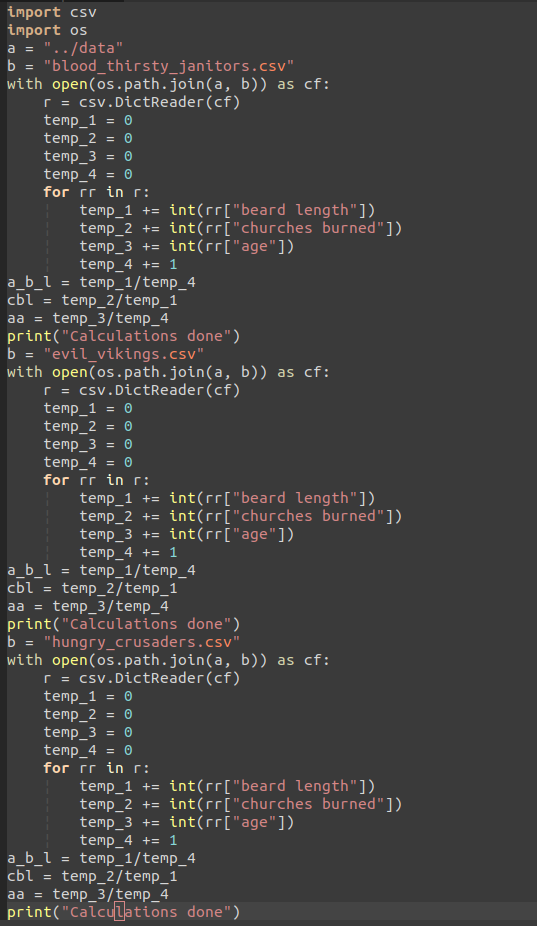
\includegraphics[width=\textwidth]{./pictures/stupid_file.png}
			\end{figure}
	\end{column}
\end{columns}
\end{frame}
\begin{frame}
	\frametitle{Using the GitHub issue tracker}
	\begin{columns}
		\begin{column}{0.5\textwidth}
			\begin{itemize}[<+->]
				\item Write a descriptive issue
				\item You can make someone responsible for fixing the issue
				\item The issue get a number you can use for referencing it
			\end{itemize}
		\end{column}
		\begin{column}{0.5\textwidth}
				\begin{figure}
					\includegraphics<1>[width=\textwidth]{./pictures/issue_created.png}
					\includegraphics<2>[width=\textwidth]{./pictures/responsible.png}
					\includegraphics<3>[width=\textwidth]{./pictures/number.png}
			\end{figure}
		\end{column}
	\end{columns}
\end{frame}
\begin{frame}
	\frametitle{Using git for fixing the code}
	\begin{columns}
		\begin{column}{0.5\textwidth}
			\begin{itemize}[<+->]
				\item Create a branch for the issue
				\item Give the branch a good name
				\item Checkout the branch
				\item We are now ready to clean up the code
				\item After the code is clean reference the issue in the commit message
				\item We can now see the commit message in GitHub
			\end{itemize}
		\end{column}
		\begin{column}{0.5\textwidth}
				\begin{figure}
					\includegraphics<1>[width=\textwidth]{./pictures/create_branch.png}
					\includegraphics<2>[width=\textwidth]{./pictures/branch_name.png}
					\includegraphics<3>[width=\textwidth]{./pictures/checkout.png}
					\includegraphics<4>[width=\textwidth]{./pictures/checkedout.png}
					\includegraphics<5>[width=\textwidth]{./pictures/issue_ref.png}
					\includegraphics<6>[width=\textwidth]{./pictures/ref_in_issue.png}
			\end{figure}
		\end{column}
	\end{columns}
\end{frame}
\begin{frame}
	\frametitle{What clean up did I do on the code}
	\begin{columns}
		\begin{column}{0.5\textwidth}
				\begin{itemize}[<+->]
					\item Added a docstring to the file
					\item Created a function
					\item Wrote a docstring for the function
					\item Added proper spacing
					\item Added comments
					\item Made reasonable variable names
				\end{itemize}
		\end{column}
		\begin{column}{0.5\textwidth}
			\begin{figure}
				\includegraphics<1>[width=\textwidth]{./pictures/module_description.png}
				\includegraphics<2>[width=\textwidth]{./pictures/function.png}
				\includegraphics<3>[width=\textwidth]{./pictures/docstring.png}
				\includegraphics<4->[width=\textwidth]{./pictures/fixed.png}
			\end{figure}
		\end{column}
	\end{columns}
\end{frame}
\begin{frame}
	\frametitle{Resolving the issue}
	\begin{columns}
		\begin{column}{0.5\textwidth}
				\begin{itemize}[<+->]
					\item The code is now clean, and we want the changes in our master branch.
					\item GitHub automatically checks if the changes are compatible.
					\item You can ask someone to review your code.
					\item After the review you can merge your code with the old.
				\end{itemize}
		\end{column}
		\begin{column}{0.5\textwidth}
			\begin{figure}
				\includegraphics<1>[width=\textwidth]{./pictures/ahead.png}
				\includegraphics<2>[width=\textwidth]{./pictures/compare.png}
				\includegraphics<3,4>[width=\textwidth]{./pictures/review.png}
			\end{figure}
		\end{column}
	\end{columns}
\end{frame}
\begin{frame}
	\frametitle{Another student downloading the changes}
	\begin{columns}
		\begin{column}{0.5\textwidth}
				\begin{itemize}[<+->]
					\item Other students can now get the changes using pull
					\item Afterwards the changes will be merged and available
				\end{itemize}
		\end{column}
		\begin{column}{0.5\textwidth}
			\begin{figure}
				\includegraphics<1>[width=\textwidth]{./pictures/pull.png}
				\includegraphics<2>[width=\textwidth]{./pictures/updated.png}
			\end{figure}
		\end{column}
	\end{columns}
\end{frame}

